\chapter{Các công trình liên quan}
\label{Chapter2}
Với sự phát triển nhanh của IoT hiện nay, những vấn đề về bảo mật, đặc biệt là trong thiết kế các kiến trúc đảm bảo tính an toàn, toàn vẹn, và quyền riêng tư của dữ liệu đang được rất quan tâm, đặt ra những bài toán cần phải giải quyết. Nghiên cứu về kiến trúc IoT không chỉ tập trung vào các giải pháp kỹ thuật như mã hóa hoặc xác thực, ngoài ra cần phải xem các thách thức thực tiễn như hạn chế tài nguyên và khả năng tương thích của thiết bị. Trong phần này, các công trình nghiên cứu liên quan sẽ được trình bày, bao gồm các mô hình, kiến trúc bảo mật IoT và các loại tấn công thường gặp, nhằm xác định những tiến bộ hiện tại, các hạn chế còn tồn tại, cũng như khoảng trống nghiên cứu mà bài luận này hướng đến.

\section{Các công trình nghiên cứu về kiến trúc IoT bảo mật}
Trước hết, bài báo trong \cite{a-decade} đã thực hiện một đánh giá toàn diện về các mô hình và kiến trúc bảo mật cho IoT. Bài báo tập trung phân tích các nghiên cứu liên quan đến bảo mật IoT trong giai đoạn từ năm 2010 đến năm 2020. Tác giả nhấn mạnh rằng lĩnh vực nghiên cứu bảo mật cho IoT vẫn còn khá mới mẻ. Các đóng góp chính trong các nghiên cứu này chủ yếu tập trung vào kiến trúc ($\sim$81\%) hoặc các mẫu ($\sim$19\%). Phần lớn các nghiên cứu đề xuất các giải pháp cụ thể, trong đó khoảng 57\% đã tiến hành kiểm thử và đánh giá ý tưởng của mình. Có khoảng 23\% các nghiên cứu đưa ra một số use case để minh họa cho ý tưởng, và chỉ khoảng 20\% bài báo triển khai thực tế một hệ thống hoàn chỉnh và thực hiện đánh giá dựa trên hệ thống đó. Ngoài ra, bài báo \cite{a-decade} cũng chỉ ra các khía cạnh bảo mật được các nghiên cứu quan tâm, bao gồm: tính bảo mật ($\sim$16\%), tính toàn vẹn ($\sim$19\%), tính khả dụng ($\sim$8\%), tính xác thực ($\sim$25\%), ủy quyền ($\sim$17\%) và quyền riêng tư ($\sim$15\%). Từ nghiên cứu trên cho thấy sự thiếu hụt trong triển khai một hệ thống thực tế. Ngoài ra, có rất nhiều khía cạnh về bảo mật cần phải quan tâm chứ không chỉ tập trung vào mỗi mã hóa dữ liệu khi triển khai một hệ thống IoT bảo mật.

Một nghiên cứu từ bài báo \cite{understandingIoT} cung cấp cái nhìn chi tiết hơn về các vấn đề bảo mật trong IoT. Bài báo giúp định nghĩa, phân loại và thảo luận về một số các thách thức về bảo mật IoT, đồng thời chỉ ra một số công trình liên quan để giải quyết các vấn đề nêu trên. Trong đó, các vấn đề chính mà bài báo đề cập bao gồm tính riêng tư trong IoT, mã hóa nhẹ, định tuyến an toàn, quản lý độ bền và khả năng phục hồi, cũng như phát hiện các cuộc tấn công từ chối dịch vụ (DoS) và tấn công nội bộ. Đặc biệt, về tính riêng tư, bài báo nhấn mạnh các thách thức như định vị trái phép, và truyền dữ liệu an toàn qua các phương tiện công cộng, đồng thời chỉ ra rằng chưa có khung công tác bảo vệ quyền riêng tư toàn diện cho nhiều ứng dụng IoT. Ngoài ra, bài báo đề xuất các giải pháp như mã hóa nhẹ và sử dụng mạng định nghĩa bởi phần mềm (SDN) để tăng cường bảo mật, nhưng việc triển khai trên các thiết bị tài nguyên thấp vẫn là một hạn chế.

Nghiên cứu của \cite{novelbased} liên quan đến bảo vệ về quyền riêng tư trong IoT, đề xuất hai giao thức bảo mật cho hệ thống chăm sóc sức khỏe dựa trên IoT, bao gồm một lược đồ xác thực dựa trên đăng nhập một lần (SSO) và một cơ chế chứng minh sự cùng tồn tại của các đối tượng gắn thẻ RF. Lược đồ SSO sử dụng hàm băm một chiều và số ngẫu nhiên để đảm bảo xác thực an toàn và truyền dữ liệu trên thiết bị tài nguyên thấp, trong khi cơ chế cùng tồn tại tăng cường an toàn bệnh nhân thông qua quản lý thuốc. Các phân tích bảo mật cho thấy các giao thức này chống lại các cuộc tấn công như giả mạo và phát lại một cách hiệu quả. Tuy nhiên, nghiên cứu chỉ mới tập trung hai giao thức riêng lẻ mà chưa tổng thể tích hợp các lớp khác nhau của hệ thống IoT, điều này này hạn chế khả năng áp dụng vào các hệ thống IoT phức tạp. Ngoài ra, các giao thức chỉ mới được đánh giá về mặt lý thuyết, nhưng không có dữ liệu về hiệu suất thực tế như thời gian xử lý, tiêu thụ năng lượng, hoặc tỷ lệ truyền thành công.

Một nghiên cứu khác là \cite{keytime} triển khai hệ thống IoT bảo mật liên quan đến chăm sóc sức khỏe. Nghiên cứu này tập trung vào quá trình tạo sinh khóa giữa máy chủ và thiết bị dựa trên dấu thời gian (Timestamp-based Secret Key Generation T-SKG) kết hợp với thuật toán DES với các chế độ ECB, CBC và CTR. Kết quả cho thấy tỷ lệ truyền gói tin khá cao từ 99.92\% đến 99.97\%. Mặc dù nghiên cứu đã triển khai một hệ thống thực tế và có các kết quả thử nghiệm, nghiên cứu này chỉ mới tập trung chủ yếu vào quá trình tạo sinh khóa chứ chưa tập trung vào phát triển một kiến trúc cụ thể. Ngoài ra, các thao tác như xác thực dữ liệu hay khả năng chống lại các cuộc tấn công vẫn chưa được phân tích một cách rõ ràng. 

Nghiên cứu của \cite{dtls} đề xuất khung bảo mật BlinkToSCoAP, tích hợp các giao thức nhẹ DTLS (Datagram Transport Layer Security), CoAP (Constrained Application Protocol), và 6LoWPAN để cung cấp bảo mật đầu cuối (end-to-end) cho các ứng dụng IoT, đặc biệt trên thiết bị hạn chế tài nguyên như cảm biến trong chăm sóc sức khỏe di động, tự động hóa tòa nhà, và lưới điện thông minh. Trong bài nghiên cứu này, nhóm tác giả trình bày các nghiên cứu lý thuyết cũng như triển khai thành công hệ thống. Các kết quả được trình bày trong bài báo cho thấy quá trình bắt tay DTLS có độ trễ trung bình là 880 ms (client) và 800 ms (server), với độ trễ lớn như vậy sẽ không phù hợp cho các ứng dụng IoT y tế yêu cầu phản hồi thời gian thực. Ngoài ra, mỗi gói tin truyền đi sẽ có thêm chi phí mỗi khung khi sử dụng DTLS và CoAP. Một nhược điểm nữa của hệ thống này đó là khóa bí mật chỉ được thiết lập một lần và sử dụng cho đến khi hết hạn, không có các cơ chế để làm mới khóa mỗi phiên mà không cần bắt tay lại, điều này có thể tăng nguy cơ bảo mật nếu khóa phiên bị xâm phạm trong thời gian dài. 

Bên cạnh các nghiên cứu đã đề cập ở trên, nhiều công trình khác cũng tập trung vào bảo mật IoT, đóng góp đáng kể vào việc phát triển các kiến trúc và giải pháp bảo mật cho IoT. Tuy nhiên, các hạn chế vẫn còn tồn tại. Phần lớn các nghiên cứu chỉ dừng ở mức lý thuyết, đề xuất các khung kiến trúc dựa trên cơ sở toán học mà thiếu triển khai thực tế. Một số nghiên cứu có thử nghiệm thực nghiệm, nhưng thường chỉ giải quyết một khía cạnh bảo mật cụ thể, như xác thực hoặc mã hóa, và hiếm có công trình nào đưa ra kiến trúc tổng quan tích hợp đa lớp. 

\section{Các mối đe dọa và loại tấn công phổ biến}
Ở phần này sẽ liệt kê một số cuộc tấn công phổ biến trong hệ thống IoT, nhằm đưa ra cái nhìn toàn diện hơn về các mối đe dọa bảo mật mà hệ thống có thể phải đối mặt trong thực tế. 
\subsection{Dò khóa bí mật của hệ thống}
Trong nhiều hệ thống IoT, việc áp dụng các thuật toán mã hóa đối xứng là cần thiết nhằm đảm bảo tính bí mật của dữ liệu trong suốt quá trình truyền tải. Tuy nhiên, nếu khóa bí mật của hệ thống bị lộ hoặc bị khai thác, kẻ tấn công có thể dễ dàng giải mã và truy cập vào nội dung dữ liệu. Do đó, trong phần này sẽ trình bày một số phương pháp tấn công phổ biến nhắm vào khóa bí mật, qua đó làm rõ các nguy cơ tiềm ẩn ảnh hưởng đến tính bảo mật của hệ thống.
\subsubsection{Tấn công brute-force}
Tấn công brute-force là phương pháp đơn giản nhất để tìm khóa bí mật trong mã hóa đối xứng, trong đó kẻ tấn công thử tất cả các tổ hợp khóa có thể cho đến khi tìm ra khóa đúng \cite{?}. Với một khóa có độ dài 40 bit, số tổ hợp khóa cần thử là \( 2^{40} \approx 1.1 \times 10^{12} \). Tùy thuộc vào thuật toán mã hóa và phần cứng sử dụng, tốc độ thử khóa của các máy tính thông thường hiện nay dao động từ \( 10^4 \) đến \( 10^9 \) khóa mỗi giây \cite{brute-force1}. 

Khi sử dụng các thiết bị phần cứng chuyên dụng như GPU (Graphics Processing Unit) cao cấp, tốc độ brute-force có thể tăng đáng kể, đạt hàng tỷ khóa mỗi giây. Một ví dụ điển hình là hệ thống do chuyên gia bảo mật Jeremi Gosney xây dựng, sử dụng 25 GPU AMD Radeon hoạt động song song thông qua nền tảng Virtual OpenCL. Hệ thống này đạt tốc độ thử nghiệm lên tới \( 3.48 \times 10^{11} \) mật khẩu NTLM mỗi giây, tương đương với khoảng \( 3.5 \times 10^{11} \) khóa mã hóa mỗi giây \cite{brute-force2}. Tương tự, dự án RC5 do Distributed.net tổ chức đã sử dụng hệ thống tính toán phân tán để giải mã dữ liệu được mã hóa bằng khóa 72 bit, đạt tốc độ brute-force lên tới \( 8 \times 10^{11} \) khóa mỗi giây \cite{brute-force3}. Những ví dụ này cho thấy sự tiến bộ đáng kể trong công nghệ brute-force, với tốc độ thử khóa ngày càng tăng nhờ vào các hệ thống phần cứng mạnh mẽ và tính toán song song.

Trong bối cảnh các hệ thống IoT, nếu thiết bị sử dụng khóa ngắn (ví dụ: 40 bit) hoặc các thuật toán mã hóa yếu như DES, khả năng bị brute-force thành công là rất cao. Tuy nhiên, điểm yếu chính của phương pháp brute-force là thời gian thực hiện. Đối với các khóa có độ dài từ 128 bit trở lên, chẳng hạn như trong thuật toán AES-128, số tổ hợp khóa cần thử là \( 2^{128} \approx 3.4 \times 10^{38} \), khiến việc brute-force trở nên bất khả thi với công nghệ hiện tại.

\subsubsection{Tấn công Side-Channel}
Tấn công Side-Channel (kênh bên) khai thác các đặc điểm vật lý hoặc hành vi của thiết bị trong quá trình thực hiện mã hóa để suy ra khóa bí mật, thay vì phân tích cấu trúc toán học của thuật toán \cite{side-channel}. Nguyên lý cơ bản là các hiệu ứng vật lý gây ra bởi hoạt động của một hệ thống mã hóa có thể cung cấp thông tin bổ sung hữu ích về các bí mật trong hệ thống, chẳng hạn như khóa mã hóa, thông tin trạng thái một phần, văn bản gốc hoàn chỉnh hoặc một phần, và những thông tin tương tự \cite{side-channel}.
% Một số loại tấn công phổ biến bao gồm:
% \begin{itemize}
%     \item Phân tích công suất: Đo tiêu thụ điện năng để suy ra khóa, gồm phân tích công suất đơn giản (SPA) và vi sai (DPA).
%     \item Phân tích điện từ: Ghi bức xạ điện từ để lấy thông tin khóa.
%     \item Tấn công thời gian: Khai thác sự khác biệt thời gian thực thi. 
%     \item Tấn công gây lỗi: Gây lỗi bằng điện áp hoặc tia laser để tạo đầu ra sai lệch.
%     \item Tấn công âm thanh: Phân tích âm thanh từ thiết bị để suy ra khóa. 
% \end{itemize}


Báo cáo từ Phòng thí nghiệm Hệ thống Nhúng, Viện Khoa học Ấn Độ , tập trung vào việc tấn công kênh bên công suất nhắm vào triển khai phần mềm của chuẩn mã hóa nâng cao (AES) trên vi điều khiển \cite{cpa} cho thấy kỹ thuật CPA có thể phá vỡ bảo mật của AES triển khai trên vi điều khiển bằng cách tiết lộ khóa bí mật. Từ đó có thể thấy ngay cả AES mạnh mẽ cũng có thể bị tấn công nếu triển khai không an toàn, đặc biệt là trên các thiết bị IoT công suất thấp.

\subsubsection{Một số cuộc tấn công dò khóa khác}
Các phương pháp cryptanalytic khai thác cấu trúc toán học của thuật toán mã hóa để tìm ra khóa bí mật hoặc giảm không gian khóa cần thử bao gồm một số phương pháp phổ biến như phân tích vi sai, phân tích tuyến tính, tấn công dựa trên plaintext đã biết (Known-Plaintext Attack - KPA) \cite{cryptanalytic}. Các phương pháp này hiệu quả đối với các thuật toán mã hóa yếu hoặc các phiên bản giảm số vòng của các thuật toán như DES. 

Tấn công related-key khai thác việc sử dụng các khóa có mối quan hệ rõ ràng (ví dụ: các khóa chỉ khác nhau một bit) để suy ra thông tin về khóa chính \cite{Related-key-attack}. Phương pháp này chỉ hiệu quả nếu hệ thống sử dụng nhiều khóa liên quan, trong các hệ thống IoT sử dụng các phương pháp tạo khóa đơn giản (như bộ đếm), tấn công related-key có thể trở nên khả thi hoặc một số thiết bị IoT có thể sử dụng các khóa liên quan để mã hóa dữ liệu giữa các thiết bị hoặc các phiên giao tiếp, tạo cơ hội cho tấn công related-key nếu triển khai không an toàn.

\subsection{Tấn công Man-in-the-Middle}
\label{sec:mitm}
Tấn công Man-in-the-Middle (MITM) là một dạng tấn công bảo mật trong đó kẻ tấn công chèn mình vào giữa hai bên giao tiếp, chẳng hạn như thiết bị IoT và máy chủ, để nghe lén, chỉnh sửa hoặc giả mạo dữ liệu mà không bị phát hiện \cite{MITM}. Từ đó, kẻ tấn công có thể bí mật thu thập dữ liệu truyền giữa các thiết bị, như khóa mã hóa hoặc thông tin nhạy cảm. 

Trong các hệ thống IoT không áp dụng mã hóa dữ liệu trước khi truyền, nguy cơ bị kẻ tấn công chặn và khai thác thông tin trên đường truyền là rất cao (Hình \ref{fig:mitm1}). Tấn công Man-in-the-Middle (MITM) đặc biệt nguy hiểm khi kẻ tấn công can thiệp vào quá trình trao đổi khóa giữa thiết bị IoT và máy chủ (Hình \ref{fig:mitm2}) \cite{mitm-dh}. Trong một số hệ thống IoT, khóa công khai được truyền trực tiếp qua kênh không an toàn. Nếu kẻ tấn công chặn được luồng giao tiếp và thay thế bằng khóa giả mạo, khóa bí mật có thể bị suy ra, dẫn đến việc hệ thống mất an toàn hoàn toàn.

\begin{figure}[h]
    \centering
    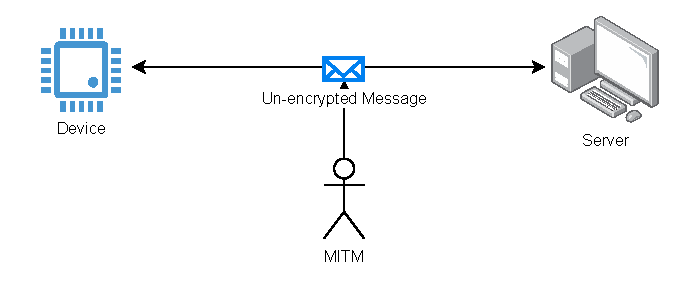
\includegraphics[width=0.7\linewidth]{images/MITM2.pdf}
    \caption{Tấn công MITM trong nghe lén dữ liệu}
    \label{fig:mitm1}
\end{figure}

\begin{figure}[h]
    \centering
    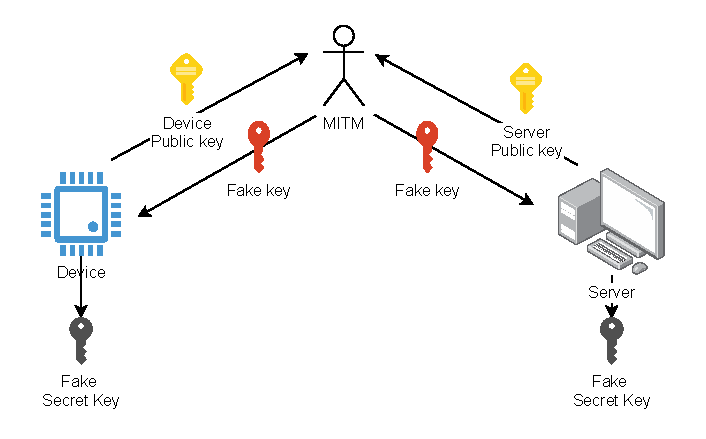
\includegraphics[width=0.7\linewidth]{images/MITM1.pdf}
    \caption{Tấn công MITM trong trao đổi khóa}
    \label{fig:mitm2}
\end{figure}

\subsection{Tấn công phát lại (Replay Attack)}
Tấn công phát lại (Replay Attack) là một dạng tấn công bảo mật trong đó kẻ tấn công chặn và ghi lại các gói tin hợp lệ từ quá trình giao tiếp giữa thiết bị IoT và máy chủ, sau đó gửi lại các gói tin này để lừa hệ thống thực hiện hành động không mong muốn, như cấp quyền truy cập trái phép hoặc thực thi lệnh giả mạo \cite{replay-attack}. Trong các hệ thống IoT, kẻ tấn công có thể ghi lại dữ liệu hợp lệ, chỉnh sửa nội dung, và gửi lại máy chủ, khiến máy chủ xử lý như gói tin hợp lệ, dẫn đến sai lệch thông tin (Hình \ref{fig:replay}). Trong các hệ thống IoT, đặc biệt là các ứng dụng thời gian thực như y tế hoặc giao thông thông minh, tấn công này đặc biệt nguy hiểm do dữ liệu sai lệch có thể gây hậu quả nghiêm trọng, ảnh hưởng trực tiếp đến an toàn và quyền lợi của người dùng.
\begin{figure}[h]
    \centering
    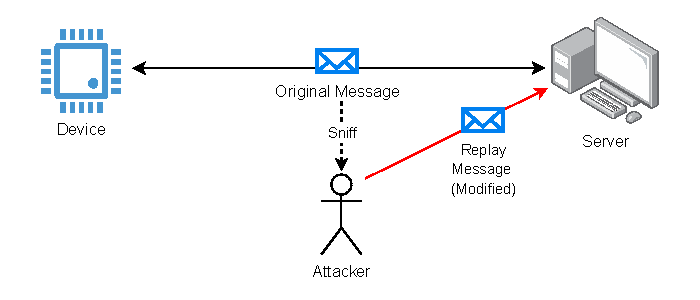
\includegraphics[width=0.7\linewidth]{images/replay.pdf}
    \caption{Minh họa cuộc tấn công phát lại}
    \label{fig:replay}
\end{figure}

\section{Khoảng trống nghiên cứu}
Dựa trên việc phân tích các ưu và nhược điểm của những nghiên cứu trước cũng như sự đa dạng và phức tạp của các hình thức tấn công vào hệ thống IoT, việc nghiên cứu và triển khai một kiến trúc bảo mật toàn diện là cần thiết và cũng là mục tiêu mà đề tài hướng đến. Bằng cách kết hợp các thuật toán mã hóa nhẹ, kiến trúc khung truyền độc lập kèm xác thực dữ liệu cùng với các phương pháp trao đổi khóa hiệu quả, đề tài hy vọng sẽ đóng góp một giải pháp có tính ứng dụng cao, đồng thời nâng cao tính bảo mật và khả năng mở rộng của hệ thống IoT trong thực tiễn.
% \section{Các phương pháp mã hóa nhẹ trong hệ thống IoT}
% (Phần này nên là lý do chọn Ascon)

% Trong các hệ thống IoT hạn chế tài nguyên, các thuật toán mã hóa truyền thống như AES hoặc RSA thường không phù hợp do yêu cầu tính toán và năng lượng cao, gây ra độ trễ lớn và tiêu tốn tài nguyên trên các thiết bị nhúng. Mã hóa nhẹ đã nổi lên như một giải pháp hiệu quả, cung cấp bảo mật mạnh mẽ với chi phí tính toán thấp. Các công trình nghiên cứu gần đây đã tập trung vào phát triển và đánh giá các thuật toán mã hóa nhẹ, chẳng hạn như Ascon và các biến thể của AES, nhằm đáp ứng nhu cầu của các ứng dụng IoT. Phần này xem xét các phương pháp mã hóa nhẹ nổi bật, làm rõ những hạn chế của chúng.

% Các công trình gần đây, chẳng hạn như bài báo Adaptive Lightweight Security for Performance Efficiency in Critical Healthcare Monitoring đã triển khai hệ thống IoT ứng dụng cho y tế đã so sánh 2 thuật toán mã hóa là Ascon-128 và AES-GCM-128 trên Raspberry Pi. Kết quả cho thấy Ascon-128 cho ra hiệu suất tốt hơn hoàn toàn so với AES-GCM-128 về mặt hiệu năng. Bài báo thực hiện so sánh tốc độ mã hóa của từng gói tin với kích thước khác nhau, Ascon cho ra hiệu suất cao với các gói tin có kích thước nhỏ, chẳng hạn với 8 byte dữ liệu, Ascon có hiệu suất gấp 8 lần so với AES và với 1024 byte, Ascon có hiệu suất gấp đôi. Với 2048 byte, Ascon vẫn cho ra hiệu suất tốt hơn dù mức độ chênh lệch không nhiều, hình \ref{fig:ascon-aes} được trích ra từ bài báo thể hiện hiệu suất của Ascon-128 so với phương pháp AES.

% \begin{figure}
%     \centering
%     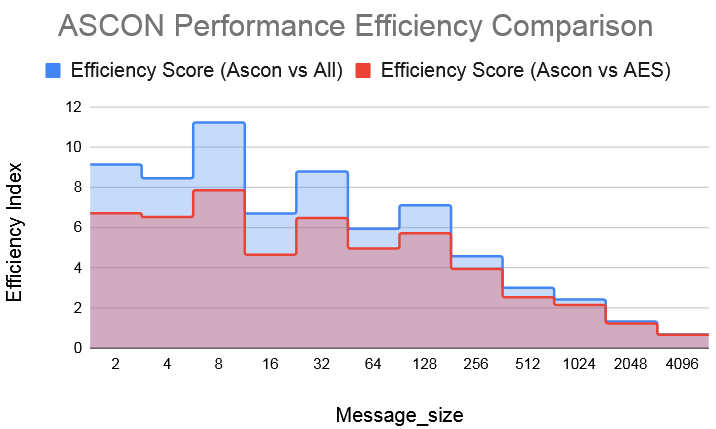
\includegraphics[width=0.8\linewidth]{ascon-aes.png}
%     \caption{Bảng so sánh hiệu năng giữa Ascon và AES được trích từ bài báo}
%     \label{fig:ascon-aes}
% \end{figure}

% Một nghiên cứu khác từ Dobraunig et al. (2021) trong bài giới thiệu Ascon v1.2 cũng nhấn mạnh hiệu suất cao của Ascon-128 khi thực hiện mã hóa dữ liệu có kích thước vừa và nhỏ so sánh với các thiết kế AES dùng native AES instruction trên Intel Skylake processors. 

% NIST cũng đã thực hiện đánh giá một số thuật toán mã hóa nhẹ ở vòng chung kết. Kết quả cho thấy Ascon là thuật toán có hiệu suất tốt nhất so với các thuật toán mã hóa nhẹ khác như Elephant, Grain-128aead hoặc Sparkle. Ascon cũng đã được NIST lựa chọn làm tiêu chuẩn mã hóa nhẹ chính thức vào năm 2023 dựa vào độ an toàn cao và hiệu suất vượt trội trên cả phần mềm lẫn phần cứng trong môi trường IoT giới hạn tài nguyên. NIST thực hiện đánh giá trên các nền tảng như 8-bit AVR, ARM Cortex-M0+/M3/M4, RISC-V, Xtensa LX6, v.v. Thời gian thực thi của Ascon nhanh hơn đáng kể so với chuẩn AES-GCM trên nRF52840. Trong các thử nghiệm benchmark độc lập, Ascon là một trong số ít thuật toán đạt hiệu suất cao và footprint nhỏ nhất, đặc biệt trên thiết bị nhúng có tài nguyên hạn chế.
% \section{Các công trình liên quan}

% Vấn đề về bảo mật trên các hệ thống IoT hạn chế tài nguyên được nghiên cứu rất nhiều trong thời gian gần đây. Các công trình nghiên cứu gần đây tập trung và nhiều biện pháp bảo mật khác nhau với nhiều kiến trúc khác nhau. Ở phần này sẽ liệt kê một số nghiên cứu và đánh giá các kiến trúc IoT đó để làm rõ những hạn chế của chúng cũng như nổi bật về nghiên cứu hiện tại của đề tài.

% \subsection{Các nghiên cứu liên quan đến ứng dụng AI trong bảo mật hệ thống IoT}

% \subsection{Các nghiên cứu liên quan đến ứng dụng mã hóa nhẹ trong đường truyền}

% \subsection{Các nghiên cứu liên quan đến trao đổi khóa mã hóa}

